\documentclass{article}

\usepackage{amsmath,amsfonts,amsthm,amssymb,amsopn,bm}
\usepackage[margin=.9in]{geometry}
\usepackage{graphicx}
\usepackage{url}
\usepackage[usenames,dvipsnames]{color}
\usepackage{fancyhdr}
\usepackage{multirow}
\usepackage{minted}
\newcommand{\field}[1]{\mathbb{#1}}
\newcommand{\1}{\mathbf{1}}
\newcommand{\E}{\mathbb{E}} 
\renewcommand{\P}{\mathbb{P}}
\newcommand{\R}{\field{R}} % real domain
% \newcommand{\C}{\field{C}} % complex domain
\newcommand{\F}{\field{F}} % functional domain

\newcommand{\T}{^{\textrm T}} % transpose

\def\diag{\text{diag}}

%% operator in linear algebra, functional analysis
\newcommand{\inner}[2]{#1\cdot #2}
\newcommand{\norm}[1]{\left\|#1\right\|}
\newcommand{\twonorm}[1]{\|#1\|_2^2}
% operator in functios, maps such as M: domain1 --> domain 2
\newcommand{\Map}[1]{\mathcal{#1}}
\renewcommand{\theenumi}{\alph{enumi}} 

\newcommand{\Perp}{\perp \! \! \! \perp}

\newcommand\independent{\protect\mathpalette{\protect\independenT}{\perp}}
\def\independenT#1#2{\mathrel{\rlap{$#1#2$}\mkern2mu{#1#2}}}
\newcommand{\vct}[1]{\boldsymbol{#1}} % vector
\newcommand{\mat}[1]{\boldsymbol{#1}} % matrix
\newcommand{\cst}[1]{\mathsf{#1}} % constant
\newcommand{\ProbOpr}[1]{\mathbb{#1}}
\newcommand{\points}[1]{\small\textcolor{magenta}{\emph{[#1 points]}} \normalsize}
\date{{}}

\setlength\parindent{0px}

\begin{document}
\title{Homework \#0}
\author{\normalsize{Spring 2020, CSE 446/546: Machine Learning}\\
\normalsize{Richy Yun} \\
\normalsize{Due: 4/8/19  11:59 PM}}
\maketitle


\section*{Probability and Statistics}
A.1 \points{2} According to the problem, we have:
\begin{center}
$p(x=1|y=1)=0.99 \qquad p(x==1|y==0)=0.01 \qquad p(y=1)=0.0001 \qquad p(y=1)=0.9999$
\end{center}
where $x=1$ is the event the test is positive, $y=1$ is the event you have the disease, and $y=1$ is the event you do not have the disease. Using Bayes rule, the probability of having the disease when you test positive is: 
\begin{center}
	$\begin{aligned}
		p(y=1|x=1)&=\dfrac{p(x=1|y=1)p(y=1)}{p(x=1|y=1)p(y=1)+p(x=1|y=0)p(y=0)}\\
		&=\dfrac{0.99\times0.001}{0.99\times0.0001+0.01\times0.9999}=0.0098
	\end{aligned}$
\end{center}

A.2 
\begin{enumerate}
\item \points{1} We can rewrite the covariance as:
\begin{center}
	$\begin{aligned}
	\text{Cov}(X,Y)&=\E[(X-\E[X])(Y-\E[Y])]\\
	&=\E[XY-Y\E[X]-X\E[Y]-\E[X]\E[Y]]\\
	&=\E[XY]-\E[Y]\E[X]-\E[X]\E[Y]-\E[X]\E[Y]\\
	&=\E[XY]-\E[X]\E[Y]
	\end{aligned}$
\end{center}

if $\E[Y|X=x]=x$ then using the law of total expectation:
\begin{center}
	$\begin{aligned}
	\E[Y|X=x]&=x\\
	\E[\E[Y|X=x]]&=\E[x]\\
	\E[Y]=\E[x]&=\E[X]
	\end{aligned}$
\end{center}
We can also rewrite $\E[XY]$ as:
\begin{center}
$\begin{aligned} \E[XY] &= \sum_{x} \sum_{y} xy p(x,y)\\
p(x,y) &= p(y|x)p(x)\\
\E[XY] &= \sum_{x} \sum_{y} xy p(y|x)p(x)\\
&=\sum_{x}xp(x)\sum_{y}yp(y|x)\\
&=\sum_{x}xp(x)\E(Y|X=x)\\
&=\sum_{x}x^2p(x)\\
&=\E[X^2]\end{aligned}$
\end{center}
Thus, we now have:
\begin{center}
$\text{Cov}(X,Y)=\E[XY]-\E[X]\E[Y]=\E[X^2]-\E[X]^2=\text{Cov}(X,X)=\E[(X-\E[X])^2]$
\end{center}


\item \points{1} From (a):
\begin{center}
	$\text{Cov}(X,Y)=\E[XY]-\E[X]\E[Y]$
\end{center}
If $X$ and $Y$ are independent, then $\E[XY]=\E[X]\E[Y]$. Thus,
\begin{center}
	$\text{Cov}(X,Y)=0$
\end{center}
\end{enumerate}


A.3 
\begin{enumerate}
	\item \points{2} To calculate the PDF you can first find the CDF and take the derivative:
	\begin{center}
		$CDF_Z(z)=p[X+Y\leq z]$
	\end{center}
	where $p$ is probability. Using the rule of total probability:
	\begin{center}
		$\begin{aligned}
		CDF_Z(z)&=\int_{-\infty}^{\infty}p[X+Y\leq z|X=x]PDF_X(x)dx\\
		&=\int_{-\infty}^{\infty}p[x+Y<=z]f(x)dx\\
		\end{aligned}$
	\end{center}
	But using the definition of CDF we can now see:
	\begin{center}
		$p[x+Y\leq z]=p[Y\leq z-x]=CDF_Y(z-x)$
	\end{center}
	Now we can take the derivative to find the PDF:
	\begin{center}
		$\begin{aligned}
		\dfrac{d}{dz}CDF_Z(z)=PDF_Z(z)=h(z)&=\dfrac{d}{dz}\int_{-\infty}^{\infty}CDF_Y(z-x)f(x)dx\\
		&=\int_{-\infty}^{\infty}\dfrac{\partial}{\partial z}CDF_Y(z-x)f(x)dx\\
		&=\int_{-\infty}^{\infty}PDF_Y(z-x)f(x)dx\\
		&=\int_{-\infty}^{\infty}g(z-x)f(x)dx
		\end{aligned}$
	\end{center}
	
	\item \points{1} The PDF of the sum of two random variables is a convolution as shown in part (a). Thus, we simply need to convolve the two uniform distributions together:
	\begin{center}
		$\begin{aligned}
		h(z)&=\int_{-\infty}^{\infty}\dfrac{\partial}{\partial z}CDF_Y(z-x)f(x)dx\\
		&=\begin{cases}
		z+1 & -1\leq z<0\\
		1-z & 0\leq z<1\\
		0 & \text{otherwise}
		\end{cases}\\
		\end{aligned}$
	\end{center}
\end{enumerate}

A.4 \points{1} $\mathcal{N}(0,1)$ indicates mean of 0 and variance of 1. With linear transformations of gaussian distributed random variables we know (from lecture and Murphy):
\begin{center}
	$\text{If} \qquad Y=aX+b, \qquad \mu_Y=a\mu_X+b \qquad \text{and} \qquad \text{var}_Y=a^2\text{var}_X$
\end{center}
where $Y$ and $X$ are gaussian distributed random variables and $a$ and $b$ are constants. Since only $a$ affects the variance, we can first find $a$ such that $\text{var}_X=1$:
\begin{center}
	$1=a^2\sigma^2 \qquad \rightarrow \qquad a=\dfrac{1}{\sigma}$
\end{center}
Next, $b$ must offset the newly scaled mean, and thus:
\begin{center}
	$0=\dfrac{1}{\sigma}\mu+b \qquad \rightarrow \qquad b=-\dfrac{1}{\sigma}\mu$
\end{center}

A.5 \points{2} If $X$ and $Y$ are independent and identically distributed, then we know (again from lecture and Murphy):
\begin{center}
	$\E[X+Y]=\E[X]+\E[Y] \qquad \text{and} \qquad \text{var}[X+Y]=\text{var}[X]+\text{var}[Y]$
\end{center}
Using these in conjunction with how the mean and variance change due to a linear transformation (as in A.4) we know:
\begin{center}
	$\text{mean}[\hat{\mu_n}]=\mu \qquad \text{and} \qquad \text{variance}[\hat{\mu_n}]=\dfrac{1}{n}\sigma^2$
\end{center}
Applying another linear transformation again changes the mean and variance, in this case $a=\sqrt{n}$ and $b=-\mu\sqrt{n}$:
\begin{center}
	$\text{mean}=a\mu+b=0 \qquad \text{and} \qquad \text{variance}=a^2\dfrac{1}{n}\sigma^2=\sigma^2$
\end{center}


A.6 
  \begin{enumerate}
  \item \points{1} The expected value of a sum of independent variables is the sum of the expected value of each random variable:
  \begin{center}
  	$\E[X+Y]=\E[X]+\E[Y]$
  \end{center}
  Thus, 
  \begin{center}
  	$\E[\hat{F_n}(x))]=\E\left [\dfrac{1}{n}\sum_{i=1}^{n}\1\{X_i\leq x\}\right ]=\dfrac{1}{n}(\E[\1\{X_1\leq x\}]+\dots+\E[\1\{X_n\leq x\}])=F(x)$
  \end{center}
  
  \item \points{1} To find the variance of $\hat{F_n}(x)$, we can first find the variance of $\1\{X_i\leq x\}$. Since it is a Bernoulli distribution, we know (from Murphy page 34):
    \begin{center}
	  	$\text{variance}[\1\{X_i\leq x\}]=\E[\1\{X_i\leq x\}](1-\E[\1\{X_i\leq x\}])=F(x)(1-F(x))$
    \end{center}
  
  	We can see that this holds true by writing out the variance:
  	\begin{center}
  		$\begin{aligned}\text{variance}[\1\{X\leq x\}]&=\E[(\1\{X\leq x\})^2]-\E[\1\{X\leq x\}]^2\\
  		&= \1\{X\leq x|X\leq x\}^2p(X\leq x) + \1\{X> x|X> x\}^2p(X> x)-F(x)^2 \\
  		&= 1\times p(X\leq x) + 0\times p(X> x)-F(x)^2\\
  		&= \1\{X\leq x|X\leq x\}p(X\leq x) -F(x)^2 \\
  		&= F(x)-F(x)^2 = F(x)(1-F(x))\end{aligned}$
    \end{center}
	Now, knowing how the variance changes due to a linear transformation, we can show:
	\begin{center}
		$\text{variance}[\hat{F_n}(x)]= \dfrac{1}{n^2} n F(x)(1-F(x))  = \dfrac{F(x)(1-F(x))}{n}$
	\end{center}
  
  \item \points{1} We first rearrange the expression:
    \begin{center}
      $\dfrac{F(x)(1-F(x))}{n} \leq \dfrac{1}{4n}$\\
      $F(x)(1-F(x)) \leq \dfrac{1}{4}$\\
      $4F(x)^2-4F(x)+1\geq0$\\
      $(2F(x)-1)^2\geq0$
    \end{center}
	Since squaring a value is always positive, the above must hold true, meaning the initial expression holds true as well.
  \end{enumerate} 

B.1  \points{1} Let $X_1,\dots,X_n$ be $n$ independent and identically distributed random variables drawn unfiromly at random from $[0,1]$. If $Y = \max\{X_1,\dots,X_n\}$ then find $\E[Y]$.\\

To calculate the expected value, we want to find the CDF then calculate the PDF:
\begin{center}
	$CDF_Y=p[\text{max}\{X_1,\dots,X_n\}\leq x]$
\end{center}
Since the maximum means everything is less than or equal to, and all $X$ are independent and identically distribtued, we can rewrite the above as:
\begin{center}
		$\begin{aligned}
	CDF_Y&=p[X_1,\dots,X_n \leq x]\\
	&=p[X_1\leq x]p[X_2\leq x]\dots p[X_n\leq x]\\
	&=\prod_{i=1}^{n}p[X_i\leq x]\\
	&=(p[X_i\leq x])^n
	\end{aligned}$
\end{center}
The PDF is then the derivative of the CDF:
\begin{center}
	$PDF_Y=\dfrac{d}{dn}(p[X_i\leq x])^n=n(p[X_i\leq x])^{n-1}$
\end{center}

$p[X_i\leq x]$ is the CDF of $X_i$. Since they are a uniform distribution from 0 to 1:
\begin{center}
	$\begin{aligned} PDF_{X_i}=\dfrac{1}{b-a}=\dfrac{1}{1-0}=1\\
	CDF_{X_i}=\int_{0}^{x}1dt=x \end{aligned}$
\end{center}
Now we can calculate the expected value using the definition, from 0 to 1 as that is the limit of the distribution:
\begin{center}
	$\begin{aligned} 
	\E[Y]=\int_{0}^{1}x\times PDF_Ydx=\int_{0}^{1}x\times n(x)^{n-1}dx&=\int_{0}^{1}n(x)^ndx\\
	&=n\dfrac{x^{n+1}}{n+1} \qquad \text{for } x=0 \text{ to } 1\\
	&=\dfrac{n}{n+1}
	\end{aligned}$
\end{center}

\section*{Linear Algebra and Vector Calculus}
A.7 
\begin{enumerate} 
	\item \points{2} The rank of both matrices is 2. For matrix $A$, the third column is three times the first column minus the second column, so there are only two linearly independent columns. For matrix $B$, the third column is the sum of the first two columns so again there are only two linearly independent columns. 
	
	\item \points{2} The basis for the column span for both matrices is the first two columns since, as mentioned above, the third column is a linear combination of the two:
	\begin{center}
		$\text{basis}=\begin{bmatrix}1 & 2 \\ 1 & 0 \\ 1 & 1 \end{bmatrix}$
	\end{center}
	
\end{enumerate}

A.8 
\begin{enumerate}
	\item \points{1} This problem requires basic matrix multiplication. The row/column of the resulting matrix is the dot product of the row from the first matrix and the column from the second. 
	\begin{center}
		$\begin{bmatrix}0&2&4 \\ 2&4&2 \\ 3&3&1 \end{bmatrix} *\begin{bmatrix}1 \\1 \\ 1 \end{bmatrix}= \begin{bmatrix} (0,2,4)\cdot(1,1,1) \\ (2,4,2)\cdot(1,1,1) \\ (3,3,1)\cdot(1,1,1) \end{bmatrix}= \begin{bmatrix}6 \\8 \\ 7 \end{bmatrix}$
	\end{center}
	\item \points{2} To solve, we need to find the inverse of matrix $A$:
	\begin{center}
		$Ax=b \qquad \rightarrow \qquad x=A^{-1}b$
	\end{center}
	First, we find the determinant both to make sure it's not 0 so it can be inverted and for use later:
	\begin{center}
		$\text{det}(A)=0(4-6)-2(2-6)+4(6-12)=-16$
	\end{center}
	Next, we transpose the matrix and find the cofactors (determinants of each minor matrix with correct signs applied):
	\begin{center}
		$A^T=\begin{bmatrix}0&2&3 \\ 2&4&3 \\ 4&2&1 \end{bmatrix}$\\
		$\text{cofactor}(A^T)=\begin{bmatrix}4-6 &2-12&4-16 \\ 2-6&0-12&0-8 \\ 6-12&0-6&0-4 \end{bmatrix} .* \begin{bmatrix}+ &-&+ \\ -&+&- \\ +&-&+ \end{bmatrix}= \begin{bmatrix}-2&10&-12 \\ 4&-12&8 \\ -6&6&-4 \end{bmatrix}$
	\end{center}
	where $.*$ represents element-wise multiplication similar to Matlab. Finally, we multiply the resulting matrix by one over the determinant:
	\begin{center}
		$A^{-1}=- \dfrac{1}{16}\begin{bmatrix}-2&10&-12 \\ 4&-12&8 \\ -6&6&-4 \end{bmatrix}= \begin{bmatrix}-0.125&-0.625&0.75 \\ -0.25&0.75&-0.5 \\ 0.375&-0.375&0.25 \end{bmatrix}$
	\end{center}
	Now we multiply $A^{-1}$ with $b$ to obtain $x$:
	\begin{center}
		$x=\begin{bmatrix}-0.125&-0.625&0.75 \\ -0.25&0.75&-0.5 \\ 0.375&-0.375&0.25 \end{bmatrix}*\begin{bmatrix}-2\\-2\\-4 \end{bmatrix} =\begin{bmatrix}-2\\1\\-1 \end{bmatrix} $
	\end{center}
	
\end{enumerate}

A.9 (Hyperplanes) Assume $w$ is an $n$-dimensional vector and $b$ is a scalar. A hyperplane in $\R^n$ is the set $\{x : x\in \R^n,\text{ s.t. } w^T x + b = 0\}$.
\begin{enumerate}
	\item \points{1} ($n=2$ example) Draw the hyperplane for $w=[-1,2]^T$, $b=2$? Label your axes.\\
	Plugging in the variables gives us a line:
	\begin{center}
		$-x_1+2x_2=-2 \qquad \rightarrow \qquad x_1-2x_2-2=0$\\
		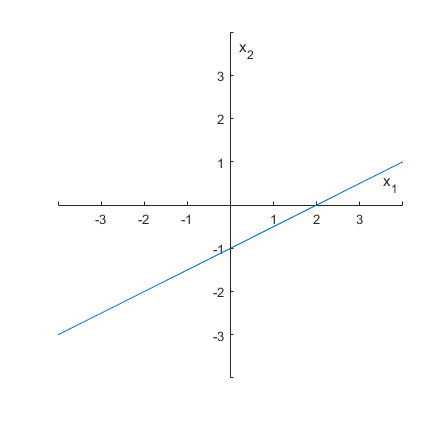
\includegraphics[width=4in]{A9a.png}
	\end{center}
	\item \points{1} ($n=3$ example) Draw the hyperplane for $w=[1,1,1]^T$, $b=0$? Label your axes.\\
	Plugging in the variables gives us a plane:
	\begin{center}
		$x_1+x_2+x_3-2=0$\\
		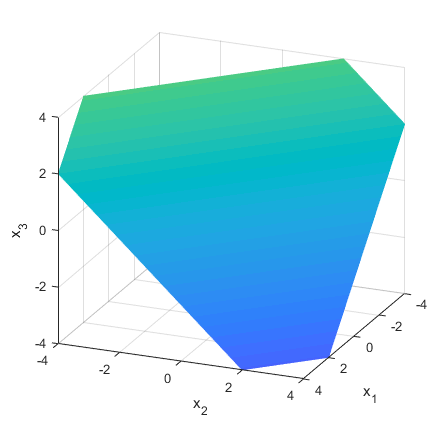
\includegraphics[width=4in]{A9b.png}
	\end{center}
	\item \points{2} Since $\widetilde{x}_0$ must fulfill $w^Tx +b = 0$, we know $w^T\widetilde{x}_0=-b$. Thus:
	\begin{center}
		$\begin{aligned}\| x_0 - \widetilde{x}_0 \| = \left | \frac{w^Tx_0 +b}{\|w\|} \right | \qquad \rightarrow \qquad \| x_0 - \widetilde{x}_0 \|^2 =  \frac{(w^Tx_0 +b)^2}{\|w\|^2} \end{aligned} $
	\end{center}
	
\end{enumerate} 

A.10 For possibly non-symmetric $\mat{A}, \mat{B} \in \R^{n \times n}$ and $c \in \R$, let $f(x, y) = x^T \mat{A} x + y^T \mat{B} x + c$. Define $\nabla_z f(x,y) = \begin{bmatrix} \frac{\partial f(x,y)}{\partial z_1} & \frac{\partial f(x,y)}{\partial z_2} & \dots & \frac{\partial f(x,y)}{\partial z_n} \end{bmatrix}^T$.  
\begin{enumerate}
	\item \points{2} Assuming $x$ and $y$ are vectors and $c$ is a constant, we know $x$ and $y$ have to be vectors of size $1\times n$ to ensure the matrix multiplication works. Therefore:
	\begin{center}
		$\begin{aligned}(\mat{A}x)_i&=\sum_{k=1}^{n}A_{ik}x_k\\
		x^T\mat{A}x&=\sum_{m=1}^{n}x_m\sum_{k=1}^{n}A_{mk}x_k=\sum_{m=1}^{n}\sum_{k=1}^{n}x_mA_{mk}x_k\\
		f(x,y)&=\sum_{m=1}^{n}\sum_{k=1}^{n}x_mA_{mk}x_k+\sum_{m=1}^{n}\sum_{k=1}^{n}y_mB_{mk}x_k+c\end{aligned}$
	\end{center}
	\item \points{2} What is $\nabla_x f(x,y)$ in terms of the summations over indices \emph{and} vector notation?\\ To approach this problem for the summation over indices, we can try thinking about what would happen element by element. For the $i$th partial derivative:
	\begin{center}
			$\begin{aligned}\nabla_{x}f(x,y)_i=\dfrac{\partial}{\partial x_i}\left(\sum_{m=1}^{n}\sum_{k=1}^{n}x_mA_{mk}x_k+\sum_{m=1}^{n}\sum_{k=1}^{n}y_mB_{mk}x_k+c\right)\end{aligned}$
	\end{center}
	We can apply the partial derivative to each part of the sum. The first term requires the product rule. Since all $x_i \neq x_1$ has a partial derivative of $0$, we can simplify the sums to just the $i$th element. Therefore we can determine the summation over indices notation:
	\begin{center}
		$\begin{aligned}\nabla_{x}f(x,y)_i&=\dfrac{\partial}{\partial x_i}\left(\sum_{m=1}^{n}\sum_{k=1}^{n}x_mA_{mk}x_k+\sum_{m=1}^{n}\sum_{k=1}^{n}y_mB_{mk}x_k+c\right)\\
		&= \dfrac{\partial}{\partial x_i}\sum_{m=1}^{n}\sum_{k=1}^{n}x_mA_{mk}x_k +  \dfrac{\partial}{\partial x_i}\sum_{m=1}^{n}\sum_{k=1}^{n}y_mB_{mk}x_k +\dfrac{\partial}{\partial x_i}c\\
		&= \sum_{m=1}^{n}\sum_{k=1}^{n}\dfrac{\partial x_m}{\partial x_i}A_{mk}x_k + \sum_{m=1}^{n}\sum_{k=1}^{n}x_mA_{mk}\dfrac{\partial x_k}{\partial x_i} + \sum_{m=1}^{n}\sum_{k=1}^{n}y_mB_{mk}\dfrac{\partial x_k}{\partial x_i}\\
		&= \sum_{k=1}^{n}A_{ik}x_k + \sum_{m=1}^{n}x_mA_{mi} + \sum_{m=1}^{n}y_mB_{mi}\end{aligned}$
	\end{center}
	We can convert this to vector notation by realizing that each sum is matrix multiplication as shown in part (a):
	\begin{center}
		$\begin{aligned}\nabla_{x}f(x,y)&= \mat{A}x+x^T\mat{A}+y^T\mat{B}\\
		&= \mat{A}x+\mat{A}^Tx+y^T\mat{B}\\
		&= \left( \mat{A}+\mat{A}^T \right)x+y^T\mat{B} \end{aligned}$
	\end{center}

	\item \points{2} What is $\nabla_y f(x,y)$ in terms of the summations over indices \emph{and} vector notation?\\
	We can approach this problem similar to part (b).
	\begin{center}
		$\begin{aligned}\nabla_{y}f(x,y)_i&=\dfrac{\partial}{\partial y_i}\left(\sum_{m=1}^{n}\sum_{k=1}^{n}x_mA_{mk}x_k+\sum_{m=1}^{n}\sum_{k=1}^{n}y_mB_{mk}x_k+c\right)\\
		&= \dfrac{\partial}{\partial y_i}\sum_{m=1}^{n}\sum_{k=1}^{n}x_mA_{mk}x_k +  \dfrac{\partial}{\partial y_i}\sum_{m=1}^{n}\sum_{k=1}^{n}y_mB_{mk}x_k +\dfrac{\partial}{\partial y_i}c\\
		&= \sum_{m=1}^{n}\sum_{k=1}^{n}\dfrac{\partial y_m}{\partial y_i}B_{mk}x_k\\
		&= \sum_{k=1}^{n}B_{ik}x_k\end{aligned}$
	\end{center}
	And again we can convert this to vector notation using matrix multiplication:
		\begin{center}
		$\begin{aligned}\nabla_{y}f(x,y)&= \mat{B}x\end{aligned}$
	\end{center}
\end{enumerate}

B.2 \points{1} The definition of matrix multiplication provides:
\begin{center}
	$\begin{aligned}AB_{ij}=\sum_{k=1}^{n}A_{ik}B_{kj}\end{aligned}$
\end{center}
Therefore, for the diagonals we have:
\begin{center}
	$\begin{aligned}AB_{ii}=\sum_{k=1}^{n}A_{ik}B_{ki}\\
	BA_{ii}=\sum_{k=1}^{n}B_{ik}A_{ki}	\end{aligned}$
\end{center}
We can rewrite the traces as:
\begin{center}
	$\begin{aligned}\text{Tr}(AB)=\sum_{i}ABii=\sum_{i=1}^{m}\sum_{k=1}^{n}A_{ik}B_{ki}\\
	\text{Tr}(BA)=\sum_{i}BAii=\sum_{i=1}^{n}\sum_{k=1}^{m}B_{ik}A_{ki}	\end{aligned}$
\end{center}
Now, simply by rearranging using the commutative property:
\begin{center}
	$\begin{aligned}\text{Tr}(AB)=\sum_{i=1}^{m}\sum_{k=1}^{n}A_{ik}B_{ki}=\sum_{i=1}^{n}\sum_{k=1}^{m}B_{ik}A_{ki}=\text{Tr}(BA)=	\end{aligned}$
\end{center}

B.3 \points{1} 
    \begin{enumerate}
        \item In the case $v_i$ has a size of $n\times 1$ the result of the product is a matrix of size $n\times n$. However, as the results of each row element is dependent on the first matrix, the product has columns that are linearly dependent with a rank of 1. Summing $n$ matrices of rank 1 results in a matrix with rank $n$ when $n<d$ and rank $d$ otherwise. 
        \item The minimum possible rank is 1 as each $v_i$ could be a linear combination of one another. The maximum possible is $n$ as long as $n< d$ and $d$ otherwise, as each vector could be linearly independent of one another, but rank cannot be larger than the smallest dimension. 
        \item First we need to determine the minimum and maximum possible rank of matrix $A$. The minimum rank is 1 as each column could be linear combinations of one column, and the maximum rank is $d$ since $D>d$. Thus, the product $Av_i$ also has a minimum and maximum rank of 1 and $d$ respectively. Although the result of $(Av_i)(Av_i^T)$ is a matrix of size $D\times D$ since $Av_i$ has maximum rank $d$ the resulting product has maximum rank $d$ similar to part (a). However, summing the matrices results in the sum of the ranks, so we end up with a matrix with a minimum rank $n$ assuming $n<D$ and a maximum rank $D$.   
        \item The rank of $AV$ depends on $A$ as mentioned in part (a). Therefore, regardless of the rank of $V$ the minimum and maximum rank of $AV$ is 1 and $d$ respectively. 
    \end{enumerate}

\section*{Programming}

A.11 
  \begin{enumerate}
  \item \points{2} \\ 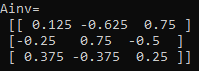
\includegraphics[width=2.25in]{A11a.png}
  \item \points{1} \\ 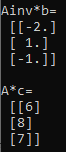
\includegraphics[width=.75in]{A11b.png}
  \end{enumerate}  

\hfill \\
A.12 \points{4} Since in problem A.6 we determined $\displaystyle \E[ ( \widehat{F}_n(x) - F(x) )^2 ] \leq \tfrac{1}{4n}$, for  $\displaystyle \sqrt{\E[ ( \widehat{F}_n(x) - F(x) )^2 ]} \leq 0.0025$, $n=40000$.
\begin{center}
	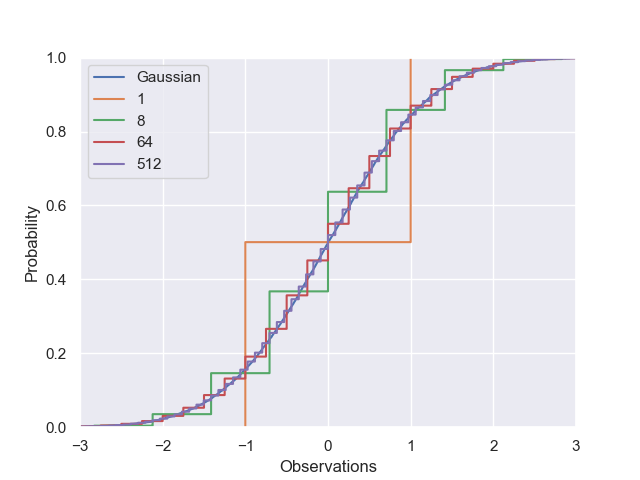
\includegraphics[width=5in]{A12.png}
\end{center} 

\section*{Source Code}

\underline{A.11} (Matlab) 
\begin{minted}{matlab}
% A9 figures
% a)
x = linspace(-5,5,100);
y = (x-2)/2;
figure; plot(x,y)
set(gca,'xaxislocation','origin')
set(gca,'yaxislocation','origin')
box off
xlim([-4,4])
ylim([-4,4])
xlabel('x_1')
ylabel('x_2')

% b)
x = linspace(-5,5,100);
y = linspace(-5,5,100);
[X,Y] = meshgrid(x,y);
Z = 2-X-Y;
figure; surf(X,Y,Z);
shading interp
set(gca,'xaxislocation','origin')
set(gca,'yaxislocation','origin')
xlim([-4,4]); ylim([-4,4]); zlim([-4,4])
xlabel('x_1'); ylabel('x_2'); zlabel('x_3');
\end{minted}

\hfill \\ 
\hfill \\
\underline{A.11} (Python)
\begin{minted}{python}

import numpy as np

# A.11 (a)
A = np.matrix('0,2,4;2,4,2;3,3,1')
Ainv = np.linalg.inv(A)
print('\nAinv=\n',Ainv)

# A.11 (b)
b = np.matrix('-2;-2;-4')
c = np.matrix('1;1;1')
print('\nAinv*b=\n',np.matmul(Ainv,b))
print('\nA*c=\n',np.matmul(A,c))
\end{minted}

\hfill \\ 
\hfill \\
\underline{A.12} (Python)
\begin{minted}{python}
import numpy as np
import matplotlib.pyplot as plt
import seaborn as sns
sns.set()

n=40000 # From problem A.6

#(a)
Z=np.random.randn(n)
plt.step(sorted(Z), np.arange(1,n+1)/float(n))

#(b)
k = [1,8,64,512]
for x in k:
Y = np.sum(np.sign(np.random.randn(n, x))*np.sqrt(1./x), axis=1)
plt.step(sorted(Y), np.arange(1,n+1)/float(n))

plt.xlim(-3,3)
plt.ylim(0,1)
plt.xlabel("Observations")
plt.ylabel("Probability")
plt.legend(['Gaussian','1','8','64','512'])	
plt.show()
\end{minted}

\end{document}
